\chapter{Valutazione dei Sistemi di Information Retrieval}
\label{chap:evaluation}

\FloatBarrier
\section{Architettura di un Motore di Ricerca}
\label{sec:architettura-motore}

Prima di affrontare la valutazione, è utile inquadrare l'architettura complessiva di un moderno motore di ricerca, che può essere schematizzata nel seguente diagramma a blocchi:

\begin{figure}[htbp]
\centering
\begin{tikzpicture}[
    node distance=1.1cm and 2.2cm,
    offline/.style={rectangle, rounded corners=4pt, draw=blue!70!black, fill=blue!8,
                    thick, minimum width=3.5cm, minimum height=0.9cm,
                    text width=3.4cm, align=center, font=\small},
    online/.style={rectangle, rounded corners=4pt, draw=teal!70!black, fill=teal!6,
                   thick, minimum width=3.5cm, minimum height=0.9cm,
                   text width=3.4cm, align=center, font=\small},
    index/.style={rectangle, rounded corners=4pt, draw=orange!80!black, fill=orange!9,
                  thick, minimum width=3.5cm, minimum height=0.9cm,
                  text width=3.4cm, align=center, font=\small},
    output/.style={rectangle, rounded corners=4pt, draw=green!60!black, fill=green!7,
                   thick, minimum width=3.5cm, minimum height=0.9cm,
                   text width=3.4cm, align=center, font=\small},
    arr/.style={-Stealth, thick},
    offcol/.style={arr, blue!70!black},
    oncol/.style={arr, teal!70!black},
    label/.style={font=\scriptsize\itshape, text=gray!70!black}
]
    %--- Colonna OFFLINE (sinistra) ---
    \node[offline] (dc)  at (0, 0)    {\textbf{Document Collection}\\{\scriptsize Web Crawler}};
    \node[offline, below=of dc]  (idx) {\textbf{Indexing}\\{\scriptsize Parsing · Tokeniz. · Stemming}};
    \node[index,   below=of idx] (ii)  {\textbf{Inverted Index}};

    %--- Colonna ONLINE (destra) ---
    \node[online,  right=3.8cm of dc]  (q)   {\textbf{Query}\\{\scriptsize Input dell'utente}};
    \node[online,  below=of q]         (qp)  {\textbf{Query Processing}\\{\scriptsize Query Expansion}};
    \node[online,  below=of qp]        (fe)  {\textbf{Feature Extraction}\\{\scriptsize BM25 · PageRank · CTR}};
    \node[online,  below=of fe]        (lr)  {\textbf{Learned Ranking (LtR)}\\{\scriptsize LambdaMART · Neural}};
    \node[output,  below=of lr]        (serp){\textbf{SERP}\\{\scriptsize Top-10 risultati all'utente}};

    %--- Etichette di colonna ---
    \node[label, above=0.25cm of dc]  {\textsc{Fase Offline}};
    \node[label, above=0.25cm of q]   {\textsc{Fase Online}};

    %--- Frecce Offline ---
    \draw[offcol] (dc.south)  -- (idx.north);
    \draw[offcol] (idx.south) -- (ii.north);

    %--- Frecce Online ---
    \draw[oncol] (q.south)   -- (qp.north);
    \draw[oncol] (qp.south)  -- (fe.north);
    \draw[oncol] (fe.south)  -- (lr.north);
    \draw[oncol] (lr.south)  -- (serp.north);

    %--- Collegamento Inverted Index → Query Processing ---
    \draw[arr, orange!80!black, dashed, thick]
        (ii.east) -- ++(0.9,0) |- (qp.west)
        node[pos=0.28, above, label] {candidate docs};

\end{tikzpicture}
\caption{Diagramma a blocchi dell'architettura di un motore di ricerca moderno: pipeline offline (indicizzazione) e pipeline online (elaborazione query e ranking).}
\label{fig:architettura-motore}
\end{figure}

I componenti principali sono:
\begin{itemize}
    \item \textbf{Web Crawler (Document Collection):} Un agente automatico che percorre il Web seguendo i collegamenti ipertestuali e scarica i documenti da indicizzare. La collezione risultante è la base di lavoro del sistema.
    \item \textbf{Indexing:} La pipeline di pre-elaborazione che trasforma i documenti grezzi in una rappresentazione indicizzabile: parsing HTML, tokenizzazione, normalizzazione, rimozione delle stopword e stemming/lemmatizzazione.
    \item \textbf{Inverted Index:} La struttura dati centrale del motore di ricerca: per ogni termine mappa la lista dei documenti che lo contengono (posting list), consentendo un recupero efficiente.
    \item \textbf{Query Processing e Query Expansion:} Il modulo che analizza la query dell'utente, la normalizza e — facoltativamente — la espande con sinonimi o termini correlati per aumentare il richiamo.
    \item \textbf{Feature Extraction:} Estrazione di segnali numerici per ciascuna coppia query-documento (TF-IDF, BM25, PageRank, freschezza, segnali di click, ecc.).
    \item \textbf{Learned Ranking Function (Learning to Rank):} Un modello statistico o di apprendimento automatico (ad es. LambdaMART, LambdaRank) addestrato a ordinare i documenti massimizzando una metrica di qualità, tipicamente NDCG.
    \item \textbf{SERP (Search Engine Results Page):} La pagina dei risultati presentata all'utente, comprensiva di titolo, snippet, URL e, nei motori moderni, risposte generate (Featured Snippets, AI Overviews).
\end{itemize}

\FloatBarrier
\section{Come Valutare la Qualità di un Motore di Ricerca}

Un sistema di Information Retrieval è un artefatto complesso che integra decine di componenti eterogenei: come si valuta qualcosa di così articolato? La risposta della comunità scientifica distingue nettamente due dimensioni complementari:

\begin{enumerate}
    \item \textbf{Metriche di Efficienza:}
    \begin{itemize}
        \item \textit{Velocità di indicizzazione:} Quanti documenti per ora il sistema è in grado di processare e inserire nell'indice.
        \item \textit{Indicizzazione incrementale:} Capacità di aggiornare l'indice con nuovi flussi documentali (ad es. $+10\,000$ prodotti al giorno in un e-commerce) senza interruzioni di servizio.
        \item \textit{Velocità di ricerca (Latenza e Throughput):} Tempo di risposta (latenza al 95° o 99° percentile) e consumo di CPU/memoria nell'elaborazione di migliaia di query al secondo su collezioni di svariati milioni o miliardi di documenti.
    \end{itemize}
    \item \textbf{Metriche di Efficacia e Qualità dei Servizi Accessori:}
    \begin{itemize}
        \item Qualità delle raccomandazioni correlate, accuratezza della correzione ortografica delle query (\textit{spell checking}) e chiarezza dei riassunti testuali visualizzati (\textit{snippet generation}).
        \item \textbf{Efficacia intrinseca della graduatoria:} Misura la capacità fondamentale del motore di ricerca di soddisfare l'utente, ordinando i documenti pertinenti nelle prime posizioni della pagina dei risultati (\textit{Search Engine Results Page}, SERP).
    \end{itemize}
\end{enumerate}

\FloatBarrier
\section{Misurare la Soddisfazione dell'Utente}

Nel contesto operativo dei motori di ricerca commerciali, l'obiettivo ultimo è massimizzare la soddisfazione dell'utente (\textit{User Happiness}). Poiché la felicità è uno stato cognitivo non osservabile direttamente, i sistemi di produzione ricorrono a proxy comportamentali online:

\begin{itemize}
    \item \textbf{Clic e Click-Through Rate (CTR):} Il numero e la proporzione di clic ricevuti dai risultati restituiti.
    \begin{itemize}
        \item \textit{Criticità:} Titoli sensazionalistici o riassunti ingannevoli (\textit{clickbait}) inducono clic elevati senza che il documento soddisfi realmente l'utente.
        \item \textit{La ricerca a zero clic (\textit{Zero-Click Search}):} L'assenza di clic non è necessariamente un segnale negativo. Quando un utente cerca informazioni fattuali (ad es. il meteo, l'orario di un volo, una conversione di valuta o una definizione enciclopedica), la risposta visualizzata direttamente tramite \textit{Featured Snippet} o \textit{Knowledge Graph} soddisfa istantaneamente il bisogno senza richiedere alcun clic.
    \end{itemize}
    \item \textbf{Conversioni e Transazioni Economiche:} Negli e-commerce, la quota di sessioni di ricerca che sfociano nell'acquisto di un prodotto e l'ammontare monetario speso dall'utente costituiscono metriche primarie di business.
    \item \textbf{Fidelizzazione e Visite Ripetute:} La percentuale di utenti che tornano ad adoperare il motore di ricerca entro un intervallo temporale predefinito (una settimana, un mese).
    \item \textbf{Dwell Time (Tempo di Permanenza):} L'intervallo di tempo che intercorre tra il momento in cui l'utente clicca su un risultato della SERP e l'istante in cui fa ritorno alla pagina dei risultati (\textit{bouncing back}). Un Dwell Time prolungato indica generalmente che il documento ha catturato l'attenzione ed è risultato informativo, mentre un ritorno immediato alla SERP denota insoddisfazione.
\end{itemize}

\begin{alertblock}{La Valutazione nell'Era dei Motori Generativi e LLM}
L'emergere di paradigmi basati su modelli linguistici (come ChatGPT, SearchGPT e Perplexity) ridefinisce radicalmente il concetto di Dwell Time e CTR: l'utente non naviga più attraverso link esterni, ma consuma sintesi testuali generate direttamente. In tale scenario, l'accuratezza fattuale, l'assenza di allucinazioni e l'attribuzione corretta delle fonti rimpiazzano il conteggio dei clic tradizionali.

Il dibattito accademico su come valutare questi sistemi è aperto e vivace. Alcune posizioni emerse in aula:
\begin{itemize}
    \item \textbf{Numero di turni conversazionali come proxy di fallimento (Dino):} In un sistema conversazionale, un elevato numero di turni necessari per soddisfare un bisogno informativo può segnalare che il sistema non ha compreso correttamente l'intento dell'utente fin dal primo scambio. Il Dwell Time classico perde di significato; si ragiona invece sulla lunghezza della conversazione.
    \item \textbf{Varianza dovuta al prompting (Gabriele):} I modelli generativi sono sensibili alla formulazione della richiesta: prompt leggermente diversi per lo stesso bisogno informativo possono produrre risposte qualitativamente molto differenti. Questa varianza intrinseca rende difficile una valutazione riproducibile.
    \item \textbf{Differenza ontologica IR classico vs.\ LLM generativo (Bruno):} Un motore classico \textit{recupera} documenti esistenti; un LLM generativo \textit{sintetizza} una risposta nuova. Si tratta di due paradigmi ontologicamente distinti: nel primo caso si può misurare la rilevanza rispetto a un corpus noto; nel secondo, l'output è unico e non confrontabile con un gold standard preesistente.
    \item \textbf{Il paradigma RAG (Retrieval-Augmented Generation):} Una risposta parziale alla critica delle allucinazioni è l'architettura RAG, che combina un motore di recupero tradizionale con un LLM generativo: si recuperano prima i documenti rilevanti dall'indice, poi si condiziona la generazione su di essi. Questo approccio riduce le allucinazioni e permette di citare le fonti, riavvicinando il sistema generativo al paradigma di valutazione classico.
\end{itemize}
\end{alertblock}

\FloatBarrier
\section{Il Paradigma di Cranfield e le Collezioni Benchmark}

Sebbene i segnali online forniscano un feedback prezioso, essi risultano rumorosi, soggetti a forti bias di posizionamento (\textit{Position Bias}) e non riproducibili sperimentalmente prima del rilascio in produzione.
Per consentire valutazioni comparative controllate, la ricerca in IR adotta il \textbf{Paradigma di Cranfield}, sviluppato originariamente da Cyril Cleverdon negli anni '60~\cite{cleverdon1967}.

È importante contestualizzare il momento storico: Cleverdon lavorava su \textbf{biblioteche fisiche}, con schedari cartacei e cataloghi aeronautici. Il suo esperimento — condotto prima dell'avvento dei calcolatori elettronici diffusi — consisteva nel valutare manualmente quanto bene diversi sistemi di classificazione documentale riuscissero a soddisfare bisogni informativi reali. Eppure, il framework metodologico che ne derivò è rimasto il fondamento della valutazione in IR per oltre sessant'anni.

\begin{definition}[Collezione di Test (Test Collection)]
Una collezione di test standard per l'Information Retrieval è una tripletta formale $\mathcal{T} = (\mathcal{D}, \mathcal{Q}, \mathcal{J})$ costituita da:
\begin{enumerate}
    \item Una collezione documentale benchmark $\mathcal{D} = \{d_1, d_2, \dots, d_N\}$;
    \item Una suite benchmark di bisogni informativi e query $\mathcal{Q} = \{q_1, q_2, \dots, q_M\}$;
    \item Un insieme di giudizi di rilevanza (\textit{Relevance Judgments} o \textit{qrels}) $\mathcal{J} = \{ (q, d) \mapsto r_{q, d} \}$, che associa a ciascuna coppia query-documento un valore di rilevanza (binario o graduato).
\end{enumerate}
\end{definition}

\subsection{La Sfida della Scalabilità Combinatoria}
La realizzazione manuale esaustiva dei giudizi di rilevanza è materialmente impossibile per archivi realistici.
Si consideri uno scenario benchmark con:
\[
|\mathcal{D}| = 5 \times 10^6 \text{ documenti}, \quad |\mathcal{Q}| = 50\,000 \text{ query}
\]
Lo spazio complessivo delle coppie ammonta a:
\[
|\mathcal{D}| \times |\mathcal{Q}| = 5 \times 10^6 \times 5 \times 10^4 = 2.5 \times 10^{11} \text{ coppie query-documento}
\]
Ipotizzando che un annotatore umano impieghi in media $2.5$ secondi per valutare la rilevanza di un documento:
\begin{align*}
\text{Tempo Totale} &= 2.5 \times 10^{11} \times 2.5\text{ s} = 6.25 \times 10^{11}\text{ secondi} \\
&\approx 173\,611\,111 \text{ ore/persona}
\end{align*}
Un impegno titanico che richiederebbe decine di migliaia di anni di lavoro umano ininterrotto!
Per ovviare a ciò, i benchmark limitano i giudizi a un sottoinsieme accuratamente campionato di documenti.

\subsection{Origini delle Query di Test}
\label{subsec:origini-query}

Una questione metodologica fondamentale riguarda la provenienza delle query che compongono il benchmark $\mathcal{Q}$:

\begin{itemize}
    \item \textbf{Motori Web commerciali — Query Logs:} I grandi motori di ricerca (Google, Microsoft Bing) campionano le query di test direttamente dai propri \textit{query log}, cioè dai log di ricerca reali degli utenti. Dataset pubblici storici come l'AOL Query Log (2006) e i dataset Microsoft ORCAS/MIMICS contengono milioni di query reali. Questo approccio garantisce che le query riflettano bisogni informativi autentici con la distribuzione di frequenza reale (incluse le query rare della coda lunga).
    \item \textbf{Scenario classico — Esperti a tavolino:} Nelle prime collezioni (Cranfield, TREC), esperti di dominio stilavano manualmente liste di \textit{information needs} plausibili, simulando i bisogni di un ipotetico utente. Il processo era deliberato e supervisionato, con attenzione a coprire diversi tipi di bisogno informativo (noto, esplorativo, transazionale).
    \item \textbf{Perché non generare query casuali dai documenti:} Una strategia apparentemente ovvia — campionare termini o frasi dai documenti della collezione per costruire query sintetiche — è metodologicamente scorretta. Le query così generate non rifletterebbero gli intenti reali degli utenti, ma solo il vocabolario dei documenti, producendo una valutazione distorta e priva di validità ecologica.
\end{itemize}

\subsection{Crowdsourcing: Opportunità e Limiti}
Una strategia economica consiste nel delegare la valutazione a lavoratori retribuiti su piattaforme online di crowdsourcing (come Amazon Mechanical Turk). Tuttavia, la letteratura scientifica evidenzia come tali giudizi siano affetti da:
\begin{itemize}
    \item Elevatissima varianza statistica;
    \item Minore competenza e presenza di spammer;
    \item Necessità di filtri rigorosi di consenso (ad es. votazione di maggioranza o calcolo dell'accordo inter-annotatore tramite coefficiente $\kappa$ di Cohen).
\end{itemize}

Una strategia più recente e sempre più diffusa è l'impiego di \textbf{LLM come Valutatori (\textit{LLM-as-a-Judge})}:
\begin{itemize}
    \item Modelli come GPT-4 vengono utilizzati con prompt strutturati per valutare la rilevanza di coppie query-documento, in sostituzione o affiancamento agli annotatori umani. La scalabilità economica è enormemente superiore al crowdsourcing tradizionale: il costo per giudizio scende di uno o due ordini di grandezza.
    \item Tuttavia, questa metodologia presenta \textbf{bias intrinseci} documentati: preferenza per testi più lunghi (indipendentemente dalla qualità), \textit{self-preference bias} (i modelli tendono a valutare meglio testi simili ai propri output di addestramento) e sensibilità all'ordine di presentazione dei candidati. È quindi necessario progettare con cura i prompt di valutazione e condurre studi di calibrazione rispetto ai giudizi umani.
\end{itemize}

\subsection{L'Infrastruttura TREC (\textit{Text REtrieval Conference})}
Promossa dal National Institute of Standards and Technology (NIST), la conferenza \textbf{TREC} rappresenta il punto di riferimento internazionale per la valutazione delle tecnologie di recupero dell'informazione.
TREC è strutturata in tracce tematiche (\textit{Tracks}), ciascuna incentrata su specifici casi d'uso (ricerca Web, ricerca clinica, domande-risposte, deep retrieval).
Il risultato prodotto da un sistema software che esegue un compito su una collezione di test prende il nome di \textbf{Run}.

La Tabella~\ref{tab:test-corpora-it} documenta l'evoluzione dimensionale delle collezioni benchmark storiche utilizzate nella ricerca in Information Retrieval~\cite{manning2008}, evidenziando il salto di scala che ha reso indispensabile la nascita di TREC.

\begin{table}[htbp]
\centering
\resizebox{\textwidth}{!}{%
\begin{tabular}{l r r r r r}
\toprule
\textbf{Collezione} & \textbf{Documenti ($N$)} & \textbf{Query} & \textbf{Dimensione (MB)} & \textbf{Termini/Doc} & \textbf{Giudizi (Q-D)} \\
\midrule
ADI & 82 & 35 & --- & --- & --- \\
AIT & 2\,109 & 14 & 2 & 400.0 & $> 10\,000$ \\
CACM & 3\,204 & 64 & 2 & 24.5 & --- \\
CISI & 1\,460 & 112 & 2 & 46.5 & --- \\
\textbf{Cranfield} & 1\,400 & 225 & 2 & 53.1 & Completi \\
LISA & 5\,872 & 35 & 3 & --- & --- \\
Medline & 1\,033 & 30 & 1 & --- & --- \\
NPL & 11\,429 & 93 & 3 & --- & --- \\
OSHMED & 348\,566 & 106 & 400 & 250.0 & 16\,140 \\
Reuters & 21\,578 & 672 & 28 & 131.0 & --- \\
\midrule
\textbf{TREC (Tipica)} & \textbf{740\,000} & \textbf{200} & \textbf{2\,000 (2 GB)} & \textbf{89--3\,543} & \textbf{$> 100\,000$} \\
\bottomrule
\end{tabular}%
}
\caption{Panoramica comparativa dei principali corpora benchmark storici di valutazione.}
\label{tab:test-corpora-it}
\end{table}

Come si evince dai dati, nelle prime collezioni degli anni '60 e '70 (come Cranfield e Medline), le ridotte dimensioni (poche migliaia di record e 1--2 MB) consentivano un'annotazione esaustiva manuale. Con l'avvento di collezioni realistiche da centinaia di migliaia di documenti e gigabyte di testo come TREC, lo spazio combinatorio delle valutazioni è esploso, imponendo l'adozione di metodologie di campionamento selettivo.

\subsection{La Tecnica del Pooling}
Per campionare i documenti da sottoporre ad annotazione umana senza dover valutare l'intera collezione, nei benchmark TREC si adotta la tecnica del \textbf{Pooling} (Figura~\ref{fig:pooling-process}):

\begin{figure}[htbp]
\centering
\begin{tikzpicture}[
    scale=0.72,
    box/.style={rectangle, rounded corners=3pt, draw=blue!80!black, fill=blue!6, thick, minimum width=2.4cm, minimum height=0.75cm, text width=2.2cm, align=center, font=\small},
    pool/.style={rectangle, rounded corners=3pt, draw=orange!80!black, fill=orange!8, thick, minimum width=3.6cm, minimum height=1.3cm, text width=3.5cm, align=center, font=\small},
    eval/.style={rectangle, rounded corners=3pt, draw=teal!80!black, fill=teal!6, thick, minimum width=3.2cm, minimum height=1.3cm, text width=3.1cm, align=center, font=\small}
]
    \node[box] (sys1) at (-0.8, 2.9) {Sistema $S_1$\\(Run 1)};
    \node[box] (sys2) at (-0.8, 1.45) {Sistema $S_2$\\(Run 2)};
    \node[box] (sysk) at (-0.8, 0.0) {Sistema $S_m$\\(Run $m$)};

    \node[pool] (poolbox) at (3.8, 1.45) {\textbf{Pool dei Candidati}\\Unione primi $k$ risultati\\$\mathcal{P} = \bigcup_{i=1}^m \text{Top-}k(S_i)$};

    \node[eval] (assess) at (9.5, 1.45) {\textbf{Giudici Umani}\\Annotazione Rilevanza\\(Relevant / Non-rel)};

    \draw[-Stealth, thick, blue!80!black] (sys1.east) -- node[above, sloped, font=\scriptsize] {Top-$k$} (poolbox.160);
    \draw[-Stealth, thick, blue!80!black] (sys2.east) -- node[above, font=\scriptsize] {Top-$k$} (poolbox.west);
    \draw[-Stealth, thick, blue!80!black] (sysk.east) -- node[below, sloped, font=\scriptsize] {Top-$k$} (poolbox.200);
    \draw[-Stealth, very thick, orange!80!black] (poolbox.east) -- node[above=3pt, font=\tiny\bfseries, text=orange!90!black] {Solo documenti in $\mathcal{P}$} (assess.west);
\end{tikzpicture}
\caption{Processo di Pooling per la selezione controllata dei documenti da annotare.}
\label{fig:pooling-process}
\end{figure}

\begin{enumerate}
    \item Si raccolgono le risposte fornite da $m$ sistemi di recupero eterogenei per una determinata query.
    \item Si estraggono i primi $k$ documenti restituiti da ciascun sistema (tipicamente $k = 50$ o $k = 100$).
    \item Si calcola l'\textbf{unione} di tali insiemi eliminando i duplicati, formando il pool $\mathcal{P}$.
    \item Gli annotatori umani valutano la rilevanza unicamente per i documenti appartenenti a $\mathcal{P}$.
\end{enumerate}

\begin{alertblock}{L'Assunzione Fondamentale del Pooling}
Tutti i documenti dell'archivio che non compaiono nel pool (\textit{unpooled}) vengono assunti convenzionalmente come \textbf{non rilevanti} ($r = 0$).
Sebbene tale assunzione introduca un potenziale bias a sfavore di algoritmi futuri con paradigmi radicalmente differenti, studi empirici condotti da NIST confermano che, a fronte di un pool formato da sistemi sufficientemente diversificati, le conclusioni comparative tra motori di ricerca rimangono stabili e affidabili.
\end{alertblock}

\FloatBarrier
\section{Bisogno Informativo vs. Query}

Una distinzione concettuale decisiva riguarda il divario tra bisogno informativo e formulazione della query:
\begin{itemize}
    \item \textbf{Bisogno Informativo (\textit{Information Need}):} Rappresenta lo stato cognitivo e l'obiettivo reale dell'utente. Ad esempio: \textit{``Il fondo della mia piscina sta diventando nero e necessita di essere ripulito''}.
    \item \textbf{Query:} L'espressione testuale sintetica digitata nel box di ricerca. Ad esempio: \texttt{``pulitore piscina''}.
\end{itemize}
\begin{property}[Principio di Valutazione della Rilevanza]
La rilevanza di un documento deve essere sempre stimata rispetto all'\textbf{Information Need} sottostante, mai rispetto alla mera sequenza di caratteri che compone la query.
\end{property}

\FloatBarrier
\section{Metriche di Valutazione Non Ordinate (\textit{Unranked Measures})}

Nel contesto del reperimento non ordinato (come nel modello booleano classico), il sistema restituisce un insieme non graduato di documenti. La valutazione si fonda sulla suddivisione dell'universo documentale mediante la matrice di contingenza (Tabella~\ref{tab:contingency-evaluation}):

\begin{table}[htbp]
\centering
\small
\begin{tabularx}{\textwidth}{l >{\centering\arraybackslash}X >{\centering\arraybackslash}X}
\toprule
& \textbf{Documento Rilevante} & \textbf{Documento Non Rilevante} \\
\midrule
\textbf{Documento Reperito} & True Positive ($TP$) & False Positive ($FP$) \\
\addlinespace
\textbf{Documento Non Reperito} & False Negative ($FN$) & True Negative ($TN$) \\
\bottomrule
\end{tabularx}
\caption{Matrice di contingenza per la classificazione binaria query-documento.}
\label{tab:contingency-evaluation}
\end{table}

\begin{figure}[htbp]
\centering
\resizebox{0.88\textwidth}{!}{%
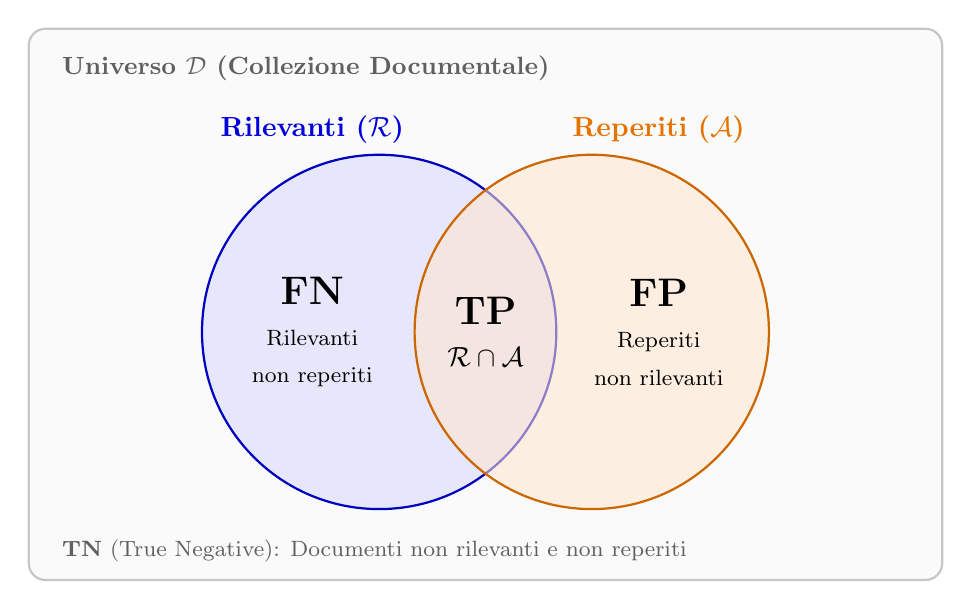
\begin{tikzpicture}
    % Document Collection Rectangle (Universe)
    \draw[thick, fill=gray!4, draw=gray!45, rounded corners=6pt] (-5.8, -3.3) rectangle (5.8, 3.7);
    \node[anchor=north west, font=\bfseries\small, text=gray!75!black] at (-5.5, 3.48) {Universo $\mathcal{D}$ (Collezione Documentale)};

    % Circles (Rilevanti e Reperiti)
    \draw[thick, fill=blue!15, draw=blue!75!black, fill opacity=0.55] (-1.35, -0.15) circle (2.25cm);
    \draw[thick, fill=orange!20, draw=orange!80!black, fill opacity=0.55] (1.35, -0.15) circle (2.25cm);

    % Circle Set Titles (Above the circles with ample margin)
    \node[font=\bfseries\normalsize, blue!85!black] at (-2.2, 2.42) {Rilevanti ($\mathcal{R}$)};
    \node[font=\bfseries\normalsize, orange!90!black] at (2.2, 2.42) {Reperiti ($\mathcal{A}$)};

    % Region Labels (Centered and well-spaced)
    \node[align=center] at (-2.2, -0.15) {\textbf{\Large FN}\\[3pt]\footnotesize Rilevanti\\[1.5pt]\footnotesize non reperiti};
    \node[align=center] at (0, -0.15) {\textbf{\Large TP}\\[3pt]\normalsize $\mathcal{R} \cap \mathcal{A}$};
    \node[align=center] at (2.2, -0.15) {\textbf{\Large FP}\\[3pt]\footnotesize Reperiti\\[1.5pt]\footnotesize non rilevanti};
    
    % True Negative label (Spacious bottom-left corner with ample clearance)
    \node[anchor=south west, font=\footnotesize, text=gray!75!black] at (-5.5, -3.2) {\textbf{TN} (True Negative): Documenti non rilevanti e non reperiti};
\end{tikzpicture}%
}
\caption{Rappresentazione insiemistica del reperimento documentale e delle regioni della matrice di confusione.}
\label{fig:venn-retrieval}
\end{figure}

\subsection{Precisione, Richiamo e loro Trade-off}
\begin{definition}[Precisione (\textit{Precision}, $P$)]
La frazione dei documenti restituiti dal sistema che risultano effettivamente rilevanti:
\begin{equation}
P = \frac{TP}{TP + FP} = P(\text{rilevante} \mid \text{reperito})
\end{equation}
\end{definition}

\begin{definition}[Richiamo (\textit{Recall}, $R$)]
La frazione dei documenti rilevanti complessivamente presenti nella collezione che il sistema è riuscito a reperire:
\begin{equation}
R = \frac{TP}{TP + FN} = P(\text{reperito} \mid \text{rilevante})
\end{equation}
\end{definition}

Esiste un intrinseco \textbf{trade-off} tra Precisione e Richiamo:
\begin{itemize}
    \item Un sistema che restituisce l'intera collezione documentale ($\text{Retrieved} = \mathcal{D}$) ottiene banalmente un richiamo perfetto $R = 100\%$, ma la sua precisione crolla a livelli minimi ($P \approx 0$).
    \item Viceversa, un sistema conservativo che restituisce unicamente il singolo documento più sicuro può conseguire $P = 100\%$, pagando il prezzo di un richiamo trascurabile.
\end{itemize}

\subsection{\texorpdfstring{La Media Armonica: F-Measure ($F_1$-Score)}{La Media Armonica: F-Measure (F1-Score)}}
Per sintetizzare Precisione e Richiamo in un unico valore scalare che premi l'equilibrio tra le due grandezze, si adotta la \textbf{F-Measure} (o $F_1$-score), definita come la \textbf{media armonica} di $P$ ed $R$:
\begin{equation}
F_1 = \frac{2}{\frac{1}{P} + \frac{1}{R}} = \frac{2 \cdot P \cdot R}{P + R} = \frac{2 \cdot TP}{2 \cdot TP + FP + FN}
\end{equation}

\begin{property}[Proprietà della Media Armonica]
La media armonica gode di proprietà matematiche fondamentali per la valutazione:
\begin{enumerate}
    \item È sempre minore o uguale alla media geometrica e alla media aritmetica:
    \[
    \frac{2}{\frac{1}{a} + \frac{1}{b}} \le \sqrt{a \cdot b} \le \frac{a + b}{2}
    \]
    \item Quando i due argomenti differiscono notevolmente, la media armonica collassa verso il \textbf{valore minimo} anziché posizionarsi a metà strada.
\end{enumerate}
\end{property}

\begin{example}[Comportamento Limite dell'F-Measure]
Si consideri un sistema banale che restituisce l'intera collezione: $R = 1.0$ e $P = 0.0001$.
\begin{itemize}
    \item La media aritmetica assegna un punteggio fuorviante pari a:
    \[
    \frac{1.0 + 0.0001}{2} \approx 0.50 \quad (50\%)
    \]
    \item La media armonica ($F_1$) demolisce giustamente la valutazione:
    \[
    F_1 = \frac{2 \cdot 1.0 \cdot 0.0001}{1.0 + 0.0001} \approx 0.0002 \quad (0.02\%)
    \]
\end{itemize}
Ciò dimostra per quale motivo la media aritmetica sia inadeguata e l'F-measure costituisca la scelta corretta.
\end{example}

\subsection{\texorpdfstring{La Misura $F_\beta$ Pesata}{La Misura F-beta Pesata}}
Qualora si desideri attribuire pesi differenziati a Precisione e Richiamo, si introduce un parametro di ponderazione $\alpha \in [0, 1]$:
\begin{equation}
F = \frac{1}{\alpha \frac{1}{P} + (1 - \alpha) \frac{1}{R}}
\end{equation}
Esprimendo $\alpha$ in funzione di un parametro $\beta$ tale che $\alpha = \frac{1}{1 + \beta^2}$, si ricava la formulazione classica di \textbf{$F_\beta$}:
\begin{equation}
F_\beta = \frac{(1 + \beta^2) \cdot P \cdot R}{\beta^2 \cdot P + R}
\end{equation}
\begin{itemize}
    \item Valori di $\beta < 1$ (ad es. $\beta = 0.5$) enfatizzano la \textbf{Precisione} rispetto al Richiamo (utile nelle ricerche su Web generico).
    \item Valori di $\beta > 1$ (ad es. $\beta = 2.0$) enfatizzano il \textbf{Richiamo} rispetto alla Precisione (fondamentale nelle ricerche brevettuali, legali e mediche, dove omettere un documento rilevante comporta danni gravi).
\end{itemize}

\FloatBarrier
\section{Metriche Basate sul Ranking (\textit{Ranked Measures} - Rilevanza Binaria)}

Nei motori di ricerca moderni i documenti non vengono restituiti come insiemi informi, ma ordinati in base a uno score di rilevanza decrescente. Inoltre, gli utenti Web raramente oltrepassano la prima pagina dei risultati (i primi $10$ o $20$ elementi).

\subsection{\texorpdfstring{Precision@k ($P@k$) e Recall@k ($R@k$)}{Precision@k e Recall@k}}
\begin{definition}[Precision@k]
Fissata una soglia di rango $k \in \mathbb{N}^+$, la Precision@k corrisponde alla proporzione di documenti rilevanti presenti nei primi $k$ posti della graduatoria:
\begin{equation}
P@k = \frac{1}{k} \sum_{i=1}^k \mathrm{rel}_i
\end{equation}
dove $\mathrm{rel}_i \in \{0, 1\}$ denota la rilevanza binaria del documento al rango $i$.
\end{definition}

\begin{example}[Calcolo di Precision@k]
Si consideri una lista ordinata in cui la sequenza di rilevanza binaria dei primi 5 documenti è data da $\langle 1, 1, 0, 0, 1 \rangle$:
\begin{itemize}
    \item $P@1 = \frac{1}{1} = 1.00$
    \item $P@2 = \frac{2}{2} = 1.00$
    \item $P@3 = \frac{2}{3} \approx 0.66$
    \item $P@4 = \frac{2}{4} = 0.50$ (si noti che $P@4 < P@3$)
    \item $P@5 = \frac{3}{5} = 0.60$
\end{itemize}
\end{example}

\begin{alertblock}{La Distorsione di $P@k$ nella Media tra Query}
Sebbene $P@k$ sia intuitivo per stimare la qualità della prima pagina, presenta un difetto metodologico critico quando viene mediato su insiemi di query eterogenee:
\begin{itemize}
    \item Se per una query specifica $q_A$ esistono solo $R_A = 2$ documenti rilevanti nell'intera collezione, il valore massimo teoricamente raggiungibile per $P@10(q_A)$ è pari a $\frac{2}{10} = 0.20$, anche qualora il motore collochi perfettamente entrambi i documenti ai primi due ranghi!
    \item Calcolando la media aritmetica di $P@10$ tra query, il motore viene ingiustamente penalizzato dalla rarità intrinseca dei documenti rilevanti di alcune query, e non da un errore dell'algoritmo di ranking.
\end{itemize}
In modo analogo, la metrica complementare $Recall@k$ ($R@k$) calcola la frazione dei documenti rilevanti complessivi reperiti entro il rango $k$:
\begin{equation}
Recall@k = \frac{1}{R} \sum_{i=1}^k \mathrm{rel}_i
\end{equation}
\end{alertblock}

\subsection{Average Precision (AP)}
L'\textbf{Average Precision} (AP) sintetizza l'intera curva Precision-Recall in un singolo indicatore scalare per una specifica query, valutando la precisione istantanea in corrispondenza di ogni posizione in cui il richiamo aumenta.

\begin{definition}[Average Precision]
Dato un ordinamento di $N$ documenti per una query con $R$ documenti rilevanti totali presenti nella collezione, l'AP è definita come:
\begin{equation}
AP = \frac{1}{R} \sum_{k=1}^N P@k \cdot \mathrm{rel}_k
\end{equation}
\end{definition}

\begin{property}[Interpretazione Geometrica e Ruolo di $1/R$]
L'Average Precision possiede una chiara interpretazione analitica:
\begin{enumerate}
    \item Ogni volta che si incontra un documento rilevante al rango $k$, il richiamo compie un gradino discreto di ampiezza $\Delta Recall = \frac{1}{R}$. L'AP calcola la somma delle aree dei rettangoli $P@k \cdot \Delta Recall$, rappresentando l'\textbf{approssimazione numerica dell'Area Sotto la Curva Precision-Recall} (AUC-PR).
    \item La normalizzazione per $R$ (il numero totale di documenti rilevanti nella collezione) garantisce che i documenti rilevanti non recuperati entro i primi $N$ ranghi contribuiscano implicitamente con precisione pari a $0$, penalizzando severamente i sistemi affetti da scarso richiamo.
\end{enumerate}
\end{property}

\begin{figure}[htbp]
\centering
\begin{tikzpicture}[
    scale=0.85,
    docrel/.style={rectangle, rounded corners=2pt, draw=teal!80!black, fill=teal!20, thick, minimum width=1.1cm, minimum height=0.65cm, font=\footnotesize\bfseries},
    docnon/.style={rectangle, rounded corners=2pt, draw=red!70!black, fill=red!10, thick, minimum width=1.1cm, minimum height=0.65cm, font=\footnotesize},
    lbl/.style={font=\scriptsize, align=center}
]
    % Document ranking blocks
    \node[lbl] at (-1.5, 0.35) {Posizione (Rango):};
    \node[lbl] at (-1.5, -0.35) {Documento:};
    \node[lbl] at (-1.5, -1.05) {Precision@k:};

    \foreach \k/\rel/\p/\type in {
        1/1/1.00/docrel,
        2/0/---/docnon,
        3/1/0.67/docrel,
        4/0/---/docnon,
        5/1/0.60/docrel%
    } {
        \node[font=\footnotesize\bfseries] at (\k*1.6, 0.35) {$k=\k$};
        \node[\type] (b\k) at (\k*1.6, -0.35) {\ifnum\rel=1 Rel\else NonRel\fi};
        \node[font=\footnotesize] at (\k*1.6, -1.05) {\ifnum\rel=1 \textbf{\p}\else \color{gray!60}--- \fi};
    }

    \draw[-Stealth, thick, blue!80!black] (0.5, 0.7) -- node[above, font=\scriptsize] {Ordinamento del Motore di Ricerca} (8.5, 0.7);
\end{tikzpicture}
\caption{Rappresentazione schematica del calcolo di Average Precision su 5 documenti con $R=3$ rilevanti totali.}
\label{fig:ap-blocks}
\end{figure}

\begin{example}[Calcolo di Base con $R=3$ Rilevanti]
Si consideri lo scenario di Figura~\ref{fig:ap-blocks} con $R=3$ documenti rilevanti totali, posizionati ai ranghi $k_1 = 1$, $k_2 = 3$ e $k_3 = 5$:
\[
P@1 = \frac{1}{1} = 1.00, \quad P@3 = \frac{2}{3} \approx 0.667, \quad P@5 = \frac{3}{5} = 0.60
\]
L'Average Precision risulta:
\begin{equation}
AP = \frac{1}{3} \left( 1.00 + \frac{2}{3} + \frac{3}{5} \right) = \frac{1}{3} \left( 2.267 \right) \approx 0.756 \quad (75.6\%)
\end{equation}
\end{example}

\begin{example}[Confronto Comparativo tra Due Ordinamenti]
Si consideri una query per la quale esistono $R = 6$ documenti rilevanti nella collezione. Due motori di ricerca alternativi restituiscono i seguenti primi 10 documenti:
\begin{itemize}
    \item \textbf{Ranking \#1:} Rilevanti concentrati nelle prime posizioni:
    \[
    \langle \text{Rel}, \text{NonRel}, \text{Rel}, \text{Rel}, \text{Rel}, \text{Rel}, \text{NonRel}, \text{NonRel}, \text{NonRel}, \text{Rel} \rangle
    \]
    \item \textbf{Ranking \#2:} Rilevanti dispersi e ritardati:
    \[
    \langle \text{NonRel}, \text{Rel}, \text{NonRel}, \text{NonRel}, \text{Rel}, \text{Rel}, \text{Rel}, \text{NonRel}, \text{Rel}, \text{Rel} \rangle
    \]
\end{itemize}
La Tabella~\ref{tab:ap-comparison} traccia l'evoluzione rango per rango di Precisione e Richiamo per entrambi i sistemi.

\begin{table}[htbp]
\centering
\resizebox{\textwidth}{!}{%
\begin{tabular}{c c c c c c c}
\toprule
& \multicolumn{3}{c}{\textbf{Ranking \#1}} & \multicolumn{3}{c}{\textbf{Ranking \#2}} \\
\cmidrule(lr){2-4} \cmidrule(lr){5-7}
\textbf{Rango ($k$)} & \textbf{Esito} & \textbf{Recall} & \textbf{Precision} & \textbf{Esito} & \textbf{Recall} & \textbf{Precision} \\
\midrule
1  & \textbf{Rel}    & 0.17 & \textbf{1.00} & NonRel          & 0.00 & --- \\
2  & NonRel          & 0.17 & ---           & \textbf{Rel}    & 0.17 & \textbf{0.50} \\
3  & \textbf{Rel}    & 0.33 & \textbf{0.67} & NonRel          & 0.17 & --- \\
4  & \textbf{Rel}    & 0.50 & \textbf{0.75} & NonRel          & 0.17 & --- \\
5  & \textbf{Rel}    & 0.67 & \textbf{0.80} & \textbf{Rel}    & 0.33 & \textbf{0.40} \\
6  & \textbf{Rel}    & 0.83 & \textbf{0.83} & \textbf{Rel}    & 0.50 & \textbf{0.50} \\
7  & NonRel          & 0.83 & ---           & \textbf{Rel}    & 0.67 & \textbf{0.57} \\
8  & NonRel          & 0.83 & ---           & NonRel          & 0.67 & --- \\
9  & NonRel          & 0.83 & ---           & \textbf{Rel}    & 0.83 & \textbf{0.56} \\
10 & \textbf{Rel}    & 1.00 & \textbf{0.60} & \textbf{Rel}    & 1.00 & \textbf{0.60} \\
\midrule
\multicolumn{2}{l}{\textbf{Average Precision (AP)}} & & \textbf{0.78} & & & \textbf{0.52} \\
\bottomrule
\end{tabular}%
}
\caption{Calcolo comparativo dettagliato di Average Precision tra Ranking \#1 e Ranking \#2.}
\label{tab:ap-comparison}
\end{table}

I rispettivi valori di AP risultano:
\begin{align*}
AP(\text{Ranking \#1}) &= \frac{1.00 + 0.67 + 0.75 + 0.80 + 0.83 + 0.60}{6} = \frac{4.65}{6} \approx \mathbf{0.78} \\
AP(\text{Ranking \#2}) &= \frac{0.50 + 0.40 + 0.50 + 0.57 + 0.56 + 0.60}{6} = \frac{3.13}{6} \approx \mathbf{0.52}
\end{align*}
Sebbene entrambi i motori raggiungano un richiamo finale identico ($R=100\%$ sui 10 documenti), Ranking \#1 ottiene un punteggio nettamente superiore ($0.78$ vs $0.52$) poiché premia la densità di documenti rilevanti nella parte alta della graduatoria.
\end{example}

\subsection{Mean Average Precision (MAP)}
Quando si valuta un motore di ricerca su un banco di prova comprendente $|\mathcal{Q}|$ bisogni informativi distinti, si calcola la \textbf{Mean Average Precision} (MAP) come media aritmetica dei valori di AP:

\begin{definition}[Mean Average Precision]
\begin{equation}
MAP = \frac{1}{|\mathcal{Q}|} \sum_{q \in \mathcal{Q}} AP(q)
\end{equation}
\end{definition}

\begin{property}[Macro-Averaging vs. Micro-Averaging]
Il MAP adotta formalmente una procedura di \textbf{Macro-Averaging}: ciascuna query possiede un peso identico pari a $1/|\mathcal{Q}|$.
\begin{itemize}
    \item Se si adottasse il \textit{Micro-Averaging} (ovvero sommare tutte le precisioni istantanee e dividere per il numero totale di documenti rilevanti dell'intera collezione), la misura verrebbe totalmente monopolizzata da pochissime query iper-generiche (ad es. \texttt{``film''} o \texttt{``notizie''}, aventi decine di migliaia di documenti rilevanti), mascherando il fallimento del motore sulle query rare e specifiche (*long-tail*).
    \item Il Macro-Averaging garantisce che ogni singola esigenza informativa dell'utente riceva pari dignità nella valutazione finale.
\end{itemize}
\end{property}

\begin{example}[Calcolo di MAP su Due Query]
Si consideri la valutazione congiunta di due query $q_1$ e $q_2$:
\begin{itemize}
    \item \textbf{Query 1 ($R_1 = 5$ rilevanti totali):} Il sistema restituisce 5 rilevanti ai ranghi $k \in \{1, 3, 6, 9, 10\}$ con precisioni istantanee pari a $1.00$, $0.67$, $0.50$, $0.44$ e $0.50$:
    \[
    AP(q_1) = \frac{1.00 + 0.67 + 0.50 + 0.44 + 0.50}{5} = \frac{3.11}{5} \approx \mathbf{0.62}
    \]
    \item \textbf{Query 2 ($R_2 = 3$ rilevanti totali):} Il sistema restituisce i 3 rilevanti ai ranghi $k \in \{2, 5, 7\}$ con precisioni istantanee pari a $0.50$, $0.40$ e $0.43$:
    \[
    AP(q_2) = \frac{0.50 + 0.40 + 0.43}{3} = \frac{1.33}{3} \approx \mathbf{0.44}
    \]
\end{itemize}
Il valore di Mean Average Precision del motore sui due compiti ammonta a:
\begin{equation}
MAP = \frac{AP(q_1) + AP(q_2)}{2} = \frac{0.62 + 0.44}{2} = \mathbf{0.53}
\end{equation}
\end{example}

\subsection{Metriche Troncate per il Web e Recommender Systems: AP@k e MAP@k}
Nei moderni motori di ricerca su Web e nei sistemi di raccomandazione, calcolare l'AP sull'intera collezione risulta impraticabile (perché il numero totale $R$ di rilevanti non è noto a priori) e poco rilevante per l'esperienza utente.
Si adotta pertanto la variante troncata a soglia fissa $K$ (\textbf{MAP@K}):

\begin{definition}[AP@K e MAP@K]
Fissata la soglia di taglio $K$ (tipicamente $K=10$ o $K=20$), l'Average Precision at $K$ per la query $q_i$ è definita come:
\begin{equation}
AP@K(q_i) = \frac{1}{K_i} \sum_{k=1}^K P@k(q_i) \cdot \mathrm{rel}(q_i, k)
\end{equation}
dove il fattore di normalizzazione $K_i$ è dato dal numero di documenti rilevanti presenti nei primi $K$ posti:
\begin{equation}
K_i = \sum_{k=1}^K \mathrm{rel}(q_i, k) \quad \left(\text{oppure } K_i = \min(R_i, K)\right)
\end{equation}
La metrica globale \textbf{MAP@K} su un insieme di query $\mathcal{Q}$ corrisponde alla media:
\begin{equation}
MAP@K(\mathcal{Q}) = \frac{1}{|\mathcal{Q}|} \sum_{q_i \in \mathcal{Q}} AP@K(q_i)
\end{equation}
\end{definition}
Questa formulazione risolve brillantemente il limite di $P@K$: normalizzando per $K_i$ anziché rigidamente per $K$, una query con soli 2 rilevanti che li colloca ai primi 2 posti ottiene $AP@10 = 1.0$ anziché essere artificialmente limitata a $0.20$.

\subsection{Mean Reciprocal Rank (MRR)}
In scenari quali le ricerche di elementi noti (\textit{Known-Item Search}), le query navigazionali (ad es. cercare l'home page di un ateneo) o il reperimento di risposte fattuali, l'utente è interessato unicamente a individuare la \textbf{prima risposta corretta}. Lo sforzo cognitivo e il tempo speso dall'utente sono inversamente proporzionali alla posizione occupata dal primo risultato rilevante:

\begin{definition}[Reciprocal Rank e MRR]
Sia $\mathrm{rank}_1(q)$ la posizione del primo documento rilevante restituito per la query $q$. Il \textbf{Reciprocal Rank} (RR) è dato da:
\begin{equation}
RR(q) = \frac{1}{\mathrm{rank}_1(q)}
\end{equation}
Il \textbf{Mean Reciprocal Rank} (MRR) è la media aritmetica su tutte le query:
\begin{equation}
MRR = \frac{1}{|\mathcal{Q}|} \sum_{q \in \mathcal{Q}} \frac{1}{\mathrm{rank}_1(q)}
\end{equation}
\end{definition}
Se per una query il primo documento rilevante si trova al rango 1, il punteggio è $1.0$; se scende al rango 2 diviene $0.5$; se scende al rango 10 crolla a $0.1$.

\FloatBarrier
\section{Oltre la Rilevanza Binaria: Rilevanza Graduata e NDCG}

Nelle applicazioni Web reali, l'ipotesi che un documento sia puramente rilevante ($1$) o non rilevante ($0$) risulta insufficiente. Si consideri la seguente query reale:
\begin{center}
\texttt{Query: ``information retrieval unipi''}
\end{center}
Una tipica SERP commerciale restituisce risultati con livelli qualitativi marcatamente differenti:
\begin{enumerate}
    \item \textbf{DidaWiki del Corso (Docente, CFU, Programma, Materiale didattico):} Rappresenta la pagina principale che soddisfa pienamente l'intento dell'utente $\implies$ \textbf{Altamente Rilevante ($r = 3$)}.
    \item \textbf{Portale Ufficiale UniPi Valutami (Scheda d'esame e requisiti istituzionali):} Pagina autorevole ma meno ricca di dispense didattiche $\implies$ \textbf{Rilevante ($r = 2$)}.
    \item \textbf{Brochure PDF del Corso di Laurea Magistrale:} Contiene solo una breve menzione del corso $\implies$ \textbf{Marginalmente Rilevante ($r = 1$)}.
    \item \textbf{Articoli di cronaca o pagine non correlate:} $\implies$ \textbf{Irrilevante ($r = 0$)}.
\end{enumerate}
Tutti i primi tre documenti sono in qualche misura attinenti, ma un utente sarà soddisfatto solo se la pagina più informativa compare in cima. Per catturare questa granularità, la letteratura adotta scale a più livelli (tipicamente $r \in \{0, 1, 2, 3\}$ o $\{0, \dots, 4\}$).

L'approccio del \textbf{Discounted Cumulative Gain} (DCG), introdotto da J\"arvelin e Kek\"al\"ainen~\cite{jarvelin2002}, poggia su due assunzioni fondamentali:
\begin{enumerate}
    \item I documenti altamente rilevanti apportano un'utilità (\textit{gain}) di gran lunga superiore rispetto a documenti solo marginalmente rilevanti.
    \item Minore è la posizione ordinale (rango) di un documento nella graduatoria, minore è la probabilità che l'utente lo esamini; pertanto, il guadagno deve essere progressivamente scontato (\textit{discounted}) verso il basso.
\end{enumerate}

\subsection{Cumulative Gain (CG) e Discounted Cumulative Gain (DCG)}
\begin{definition}[Cumulative Gain a Rango $p$]
Dato il vettore delle rilevanze graduate $\mathbf{r} = [r_1, r_2, \dots, r_p]$, il Cumulative Gain è la somma lineare dei guadagni:
\begin{equation}
CG_p = \sum_{i=1}^p r_i
\end{equation}
Il $CG_p$ è insensibile alla posizione: scambiare un documento altamente rilevante al rango 1 con uno al rango 10 non altera il valore di $CG_p$.
\end{definition}

\begin{definition}[Discounted Cumulative Gain (Formulazione Standard)]
Il DCG applica uno sconto logaritmico basato sul rango della posizione $i$:
\begin{equation}
DCG_p = r_1 + \sum_{i=2}^p \frac{r_i}{\log_2(i)}
\label{eq:dcg-standard-it}
\end{equation}
\end{definition}

\begin{alertblock}{Significato Comportamentale dello Sconto Logaritmico}
Lo sconto $\frac{1}{\log_2(i)}$ riflette il decadimento esponenziale dell'attenzione visiva dell'utente secondo il modello di lettura a cascata:
\begin{itemize}
    \item Al rango $i = 4$, il fattore di sconto è $\frac{1}{\log_2(4)} = \frac{1}{2}$: il valore informativo percepito si dimezza rispetto alla prima posizione.
    \item Al rango $i = 8$, il fattore è $\frac{1}{\log_2(8)} = \frac{1}{3}$.
    \item Al rango $i = 16$, il fattore scende a $\frac{1}{\log_2(16)} = \frac{1}{4}$.
\end{itemize}
\end{alertblock}

Nei motori di ricerca commerciali (Google, Bing) si impiega frequentemente la \textbf{formulazione esponenziale}:
\begin{equation}
DCG_p^{\text{exp}} = \sum_{i=1}^p \frac{2^{r_i} - 1}{\log_2(i + 1)}
\label{eq:dcg-exp-it}
\end{equation}
\begin{noteblock}{Chiarimento sulla Notazione degli Indici}
Si noti la differenza nell'argomento del logaritmo:
\begin{itemize}
    \item Nell'Equazione~\eqref{eq:dcg-standard-it} il primo termine $r_1$ viene estratto per evitare $\log_2(1) = 0$ al denominatore, mentre la sommatoria parte da $i=2$ con $\log_2(i)$.
    \item Nell'Equazione~\eqref{eq:dcg-exp-it} la sommatoria include direttamente il rango $i=1$ adottando $\log_2(i+1)$ al denominatore ($\log_2(1+1) = \log_2(2) = 1$).
    \item Inoltre, il numeratore $2^{r_i} - 1$ enfatizza in modo non lineare i documenti di massima rilevanza ($r=3 \implies 2^3 - 1 = 7$, mentre $r=1 \implies 2^1 - 1 = 1$), penalizzando aspramente il loro mancato posizionamento nei primi ranghi.
\end{itemize}
\end{noteblock}

\subsection{Normalized Discounted Cumulative Gain (NDCG)}
Poiché query differenti presentano un numero variabile di documenti rilevanti, il valore grezzo di $DCG_p$ non è confrontabile tra query diverse. Si ricorre quindi all'\textbf{Ideal DCG} ($IDCG_p$), ottenuto calcolando il DCG della graduatoria ideale che ordina tutti i documenti per rilevanza decrescente:
\begin{equation}
NDCG_p = \frac{DCG_p}{IDCG_p} \quad \in [0, 1]
\end{equation}

\subsection{Esempio Numerico Completo: Calcolo Passo-Passo}
Si consideri la seguente graduatoria di 10 documenti, valutati su scala $0$--$3$:
\[
\mathbf{r} = [3, \, 2, \, 3, \, 0, \, 0, \, 1, \, 2, \, 2, \, 3, \, 0]
\]
La sequenza ideale ottenuta ordinando per rilevanza non crescente è:
\[
\mathbf{r}^* = [3, \, 3, \, 3, \, 2, \, 2, \, 2, \, 1, \, 0, \, 0, \, 0]
\]
La Tabella~\ref{tab:ndcg-step-by-step} riporta l'evoluzione dettagliata di ogni singolo termine posizionale.

\begin{table}[htbp]
\centering
\resizebox{\textwidth}{!}{%
\begin{tabular}{c c l c >{\bfseries}c c c >{\bfseries}c >{\bfseries}c}
\toprule
$i$ & $r_i$ & Sconto & Guadagno Scontato & $DCG@i$ & $r_i^*$ & Guadagno Ideale & $IDCG@i$ & $NDCG@i$ \\
\midrule
1 & 3 & 1.000 & 3.00 & 3.00 & 3 & 3.00 & 3.00 & 1.00 \\
2 & 2 & $\log_2(2) = 1.000$ & 2.00 & 5.00 & 3 & 3.00 & 6.00 & 0.83 \\
3 & 3 & $\log_2(3) = 1.585$ & 1.89 & 6.89 & 3 & 1.89 & 7.89 & 0.87 \\
4 & 0 & $\log_2(4) = 2.000$ & 0.00 & 6.89 & 2 & 1.00 & 8.89 & 0.76 \\
5 & 0 & $\log_2(5) = 2.322$ & 0.00 & 6.89 & 2 & 0.86 & 9.75 & 0.71 \\
6 & 1 & $\log_2(6) = 2.585$ & 0.39 & 7.28 & 2 & 0.77 & 10.52 & 0.69 \\
7 & 2 & $\log_2(7) = 2.807$ & 0.71 & 7.99 & 1 & 0.36 & 10.88 & 0.73 \\
8 & 2 & $\log_2(8) = 3.000$ & 0.67 & 8.66 & 0 & 0.00 & 10.88 & 0.80 \\
9 & 3 & $\log_2(9) = 3.170$ & 0.95 & 9.61 & 0 & 0.00 & 10.88 & 0.88 \\
10 & 0 & $\log_2(10) = 3.322$ & 0.00 & 9.61 & 0 & 0.00 & 10.88 & 0.88 \\
\bottomrule
\end{tabular}%
}
\caption{Tracciamento dettagliato del calcolo di $DCG@i$, $IDCG@i$ e $NDCG@i$ per $i=1,\dots,10$.}
\label{tab:ndcg-step-by-step}
\end{table}

\subsection{Confronto tra Funzioni di Ranking Alternative}
Si consideri il caso studio di 4 documenti $\{d_1, d_2, d_3, d_4\}$ con gradi di rilevanza:
\[
r(d_1) = 0, \quad r(d_2) = 1, \quad r(d_3) = 2, \quad r(d_4) = 2
\]
\begin{itemize}
    \item \textbf{Ground Truth ($GT$):} Ordinamento $\langle d_4, d_3, d_2, d_1 \rangle$ con vettori di rilevanza $[2, 2, 1, 0]$:
    \begin{align*}
    IDCG_4 &= 2 + \frac{2}{\log_2(2)} + \frac{1}{\log_2(3)} + 0 = 2 + 2 + 0.6309 = 4.6309 \\
    NDCG_{GT} &= 1.00
    \end{align*}
    \item \textbf{Ranking Function 1 ($RF_1$):} Ordinamento $\langle d_3, d_4, d_2, d_1 \rangle$ con rilevanze $[2, 2, 1, 0]$.
    Poiché i primi due documenti possiedono il medesimo grado ($r=2$), l'inversione non produce alcuna penalità posizionale:
    \begin{align*}
    DCG_{RF_1} &= 2 + \frac{2}{\log_2(2)} + \frac{1}{\log_2(3)} = 4.6309 \\
    NDCG_{RF_1} &= \frac{4.6309}{4.6309} = 1.00
    \end{align*}
    \item \textbf{Ranking Function 2 ($RF_2$):} Ordinamento $\langle d_3, d_2, d_4, d_1 \rangle$ con rilevanze $[2, 1, 2, 0]$.
    In questo caso, il documento $d_2$ ($r=1$) scavalca erroneamente $d_4$ ($r=2$):
    \begin{align*}
    DCG_{RF_2} &= 2 + \frac{1}{\log_2(2)} + \frac{2}{\log_2(3)} + 0 = 2 + 1 + \frac{2}{1.585} = 4.2619 \\
    NDCG_{RF_2} &= \frac{DCG_{RF_2}}{IDCG_4} = \frac{4.2619}{4.6309} \approx 0.9203
    \end{align*}
\end{itemize}
Questo calcolo dimostra con precisione matematica come la metrica NDCG penalizzi le inversioni di rango proporzionalmente alla gravità dello scambio di rilevanza.
